%%%%%%%%%%%%%%%%%%%%%%%%%%%%%%%%%%%%%%%%%%%%%%%%%%%%%%%%%%%%%%%%%
\chapter{FLOW PREDICTION}\label{ch:fp}
%%%%%%%%%%%%%%%%%%%%%%%%%%%%%%%%%%%%%%%%%%%%%%%%%%%%%%%%%%%%%%%%%

\vspace{-12pt} %iki başlık alt alta. iki katı boşluk olmasın

\section{Purpose}

Lorem ipsum dolor sit amet, consectetur adipiscing elit. Sed ac augue vel dui 
adipiscing placerat et nec metus. Donec bibendum sodales mollis. Cras in lacus 
justo, at vestibulum quam. Sed semper, est sit amet consectetur ornare, leo est 
lacinia velit, adipiscing elementum lectus felis at sem. Aenean hendrerit erat eu 
lacus malesuada at sodales arcu egestas. Maecenas euismod urna ut sem luctus et 
congue metus vulputate. Ut pellentesque, neque eget fringilla elementum, ligula 
massa aliquet lorem, et varius nisi lacus vel diam. Etiam vitae metus sed orci 
rutrum fringilla. Phasellus sed velit quam. Mauris vestibulum, mauris a cursus 
adipiscing, nulla est hendrerit justo, ut fringilla eros velit ut mauris.

\begin{itemize}[itemsep=0pt, parsep=6pt, topsep=6pt]
	\item{Figures, tables can be enlarged and be reduced.}
	\item{The explanations except from the first reference about the figure or table can be placed either before the figure/table or after.}
	\item{After referring to a figure or table it is placed to the closest and convenient location. Convenient location must be arranged considering the gap at the bottom of the page.}
\end{itemize}

Sed et est vestibulum felis sagittis congue. Phasellus fringilla sem eu purus 
posuere ut viverra massa dignissim. Maecenas ornare neque velit. Vivamus interdum 
euismod elementum. Ut sit amet luctus ligula. Vivamus porttitor venenatis sem nec 
congue. Quisque sed lectus et nibh imperdiet vestibulum. Vivamus vel turpis leo. 
Proin suscipit iaculis nibh, nec dictum augue aliquet in. Praesent fermentum sem 
tempus orci molestie at facilisis dui sagittis. Etiam sit amet imperdiet sapien. 

\subsection{Artificial neural networks}

Lorem ipsum dolor sit amet, consectetur adipiscing elit. Sed ac augue vel dui 
adipiscing placerat et nec metus. Donec bibendum sodales mollis. Cras in lacus 
justo, at vestibulum quam. Sed semper, est sit amet consectetur ornare, leo est 
lacinia velit, adipiscing elementum lectus felis at sem. Aenean hendrerit erat eu 
lacus malesuada at sodales arcu egestas. Maecenas euismod urna ut sem luctus et 
congue metus vulputate Figure \ref{fig:Ch3-1-1}.

\vspace{6pt}
\begin{figure}[ht]
      \centering
      
\includegraphics[width=230pt,keepaspectratio=true]{./fig/sekil3}
      % sekil3.eps: 0x0 pixel, 300dpi, 0.00x0.00 cm, bb=14 14 1155 740
      \caption[Short version for LoF]{Long version to appear next to the figure.}
      \label{fig:Ch3-1}
\end{figure}
\vspace{-6pt}

Lorem ipsum dolor sit amet, consectetur adipiscing elit. Sed ac augue vel dui 
adipiscing placerat et nec metus. Donec bibendum sodales mollis. Cras in lacus 
justo, at vestibulum quam. Sed semper, est sit amet consectetur ornare, leo est 
lacinia velit, adipiscing elementum lectus felis at sem. Aenean hendrerit erat eu 
lacus malesuada at sodales arcu egestas. Maecenas euismod urna ut sem luctus et 
congue metus vulputate. Ut pellentesque, neque eget fringilla elementum, ligula 
massa aliquet lorem, et varius nisi lacus vel diam. Etiam vitae metus sed orci 
rutrum fringilla. Phasellus sed velit quam. Mauris vestibulum, mauris a cursus 
adipiscing, nulla est hendrerit justo, ut fringilla eros velit ut mauris.

Sed et est vestibulum felis sagittis congue. Phasellus fringilla sem eu purus 
posuere ut viverra massa dignissim. Maecenas ornare neque velit. Vivamus interdum 
euismod elementum. Ut sit amet luctus ligula. Vivamus porttitor venenatis sem nec 
congue. Quisque sed lectus et nibh imperdiet vestibulum. Vivamus vel turpis leo. 
Proin suscipit iaculis nibh, nec dictum augue aliquet in. Praesent fermentum sem 
tempus orci molestie at facilisis dui sagittis. Etiam sit amet imperdiet sapien.

\subsection{Autoregressive models}

Lorem ipsum dolor sit amet, consectetur adipiscing elit. Sed ac augue vel dui 
adipiscing placerat et nec metus. Donec bibendum sodales mollis. Cras in lacus 
justo, at vestibulum quam. Sed semper, est sit amet consectetur ornare, leo est 
lacinia velit, adipiscing elementum lectus felis at sem. Aenean hendrerit erat eu 
lacus malesuada at sodales arcu egestas. Maecenas euismod urna ut sem luctus et 
Equation \eqref{eq:Ch3-1}.
% 6pt boşluk için satır atlanmaması lazım
\begin{equation}
\label{eq:Ch3-1}
   y_{t}  \equiv \phi_{1} y_{t-1} + \epsilon_{t}
\end{equation}

Congue metus vulputate. Ut pellentesque, neque eget fringilla elementum, ligula 
massa aliquet lorem, et varius nisi lacus vel diam. Etiam vitae metus sed orci 
rutrum fringilla. Phasellus sed velit quam. Mauris vestibulum, mauris a cursus 
adipiscing, nulla est hendrerit justo, ut fringilla eros velit ut mauris.

\subsection{Process based model: SWAT}

Lorem ipsum dolor sit amet, consectetur adipiscing elit. Sed ac augue vel dui 
adipiscing placerat et nec metus. Donec bibendum sodales mollis. Cras in lacus 
justo, at vestibulum quam. Sed semper, est sit amet consectetur ornare, leo est 
lacinia velit, adipiscing elementum lectus felis at sem. Aenean hendrerit erat eu 
lacus malesuada at sodales arcu egestas. Maecenas euismod urna ut sem luctus et 
congue metus vulputate. Ut pellentesque, neque eget fringilla elementum, ligula 
massa aliquet lorem, et varius nisi lacus vel diam. Etiam vitae metus sed orci 
rutrum fringilla. Phasellus sed velit quam. Mauris vestibulum, mauris a cursus 
adipiscing, nulla est hendrerit justo, ut fringilla eros velit ut mauris.

Fİg. \ref{fig:ch3-2} Sed et est vestibulum felis sagittis congue. Phasellus fringilla sem eu purus 
posuere ut viverra massa dignissim. Maecenas ornare neque velit. Vivamus interdum 
euismod elementum. Ut sit amet luctus ligula. Vivamus porttitor venenatis sem nec 
congue. Quisque sed lectus et nibh imperdiet vestibulum. Vivamus vel turpis leo. 
Proin suscipit iaculis nibh, nec dictum augue aliquet in. Praesent fermentum sem 
tempus orci molestie at facilisis dui sagittis. Etiam sit amet imperdiet sapien.

\vspace{6pt}
\begin{figure}[h!]
      \centering
      
\includegraphics[width=230pt,keepaspectratio=true]{./fig/sekil3}
      % sekil3.eps: 0x0 pixel, 300dpi, 0.00x0.00 cm, bb=14 14 1155 740
      \vspace{4mm}
      \caption{For a multi-line figure captions, it is important that all the
      lines of the caption are aligned.}
      \label{fig:ch3-2}
\end{figure}
\vspace{-6pt}

Lorem ipsum dolor sit amet, consectetur adipiscing elit. Sed ac augue vel dui 
adipiscing placerat et nec metus. Donec bibendum sodales mollis. Cras in lacus 
justo, at vestibulum quam. Sed semper, est sit amet consectetur ornare, leo est 
lacinia velit, adipiscing elementum lectus felis at sem. Aenean hendrerit erat eu 
lacus malesuada at sodales arcu egestas. Maecenas euismod urna ut sem luctus et 
congue metus vulputate. Ut pellentesque, neque eget fringilla elementum, ligula 
massa aliquet lorem, et varius nisi lacus vel diam. Etiam vitae metus sed orci 
rutrum fringilla. Phasellus sed velit quam. Mauris vestibulum, mauris a cursus 
adipiscing, nulla est hendrerit justo, ut fringilla eros velit ut mauris.

Sed et est vestibulum felis sagittis congue. Phasellus fringilla sem eu purus 
posuere ut viverra massa dignissim. Maecenas ornare neque velit. Vivamus interdum 
euismod elementum. Ut sit amet luctus ligula. Vivamus porttitor venenatis sem nec 
congue. Quisque sed lectus et nibh imperdiet vestibulum. Vivamus vel turpis leo. 
Proin suscipit iaculis nibh, nec dictum augue aliquet in. Praesent fermentum sem 
tempus orci molestie at facilisis dui sagittis. Etiam sit amet imperdiet sapien.

\subsection{Multi variable analysis}

Lorem ipsum dolor sit amet, consectetur adipiscing elit. Sed ac augue vel dui 
adipiscing placerat et nec metus. Donec bibendum sodales mollis. Cras in lacus 
justo, at vestibulum quam. Sed semper, est sit amet consectetur ornare, leo est 
lacinia velit, adipiscing elementum lectus felis at sem. Aenean hendrerit erat eu 
lacus malesuada at sodales arcu egestas. Maecenas euismod urna ut sem luctus et 
congue metus vulputate. Ut pellentesque, neque eget fringilla elementum, ligula 
massa aliquet lorem, et varius nisi lacus vel diam. Etiam vitae metus sed orci 
rutrum fringilla. Phasellus sed velit quam. Mauris vestibulum, mauris a cursus 
adipiscing, nulla est hendrerit justo, ut fringilla eros velit ut mauris.

Sed et est vestibulum felis sagittis congue. Phasellus fringilla sem eu purus 
posuere ut viverra massa dignissim. Maecenas ornare neque velit. Vivamus interdum 
euismod elementum. Ut sit amet luctus ligula. Vivamus porttitor venenatis sem nec 
congue. Quisque sed lectus et nibh imperdiet vestibulum. Vivamus vel turpis leo. 
Proin suscipit iaculis nibh, nec dictum augue aliquet in. Praesent fermentum sem 
tempus orci molestie at facilisis dui sagittis. Etiam sit amet imperdiet sapien 
Fig \ref{fig:ch3-3}

\vspace{6pt}
\begin{figure}[h!]
 \centering
 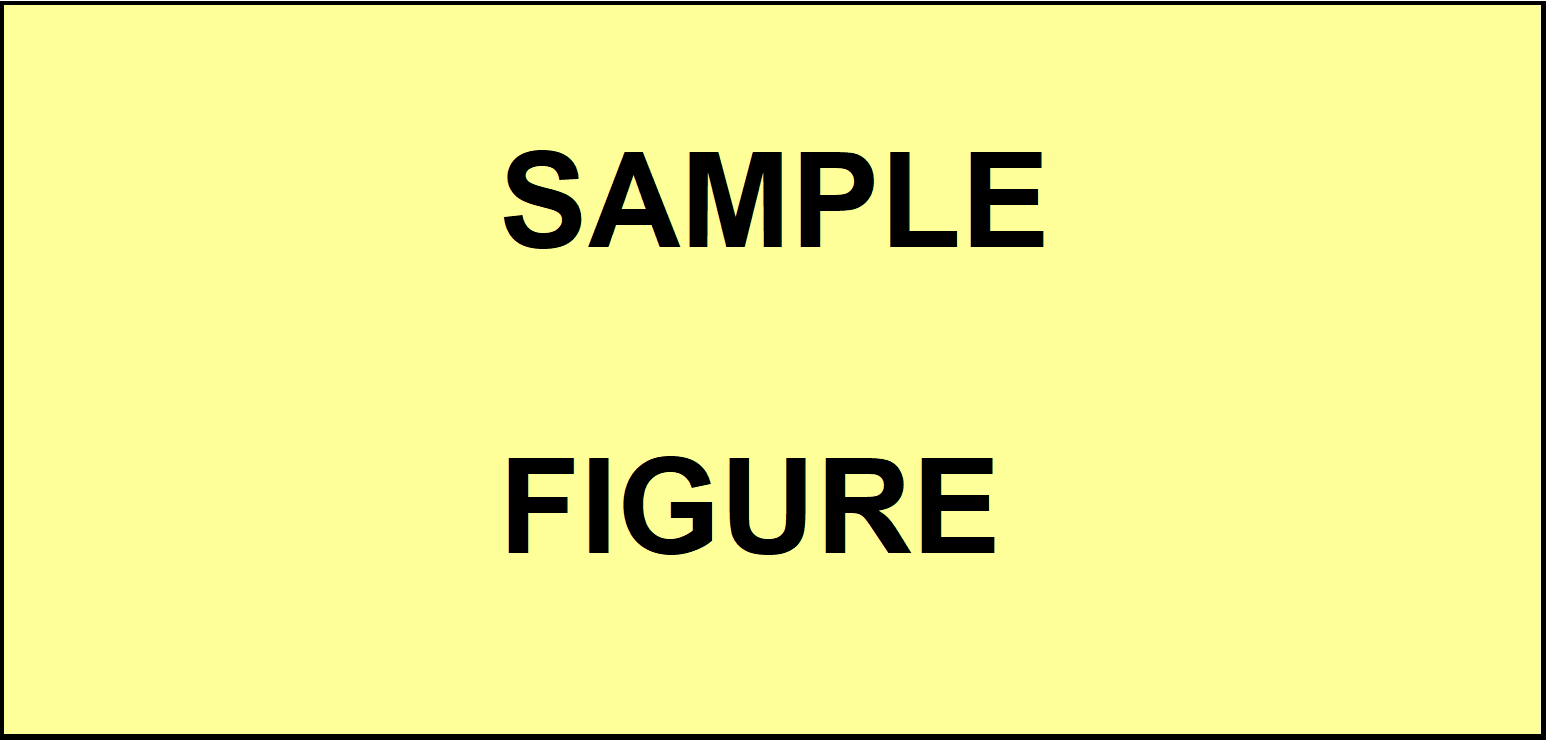
\includegraphics[width=290pt,keepaspectratio=true]{./fig/sekil4}
 % sekil4.eps: 0x0 pixel, 300dpi, 0.00x0.00 cm, bb=14 14 1148 603
 \caption{Figure captions must be ended with a full stop.}
 \label{fig:ch3-3}
\end{figure}
\vspace{-6pt}

Lorem ipsum dolor sit amet, consectetur adipiscing elit. Sed ac augue vel dui 
adipiscing placerat et nec metus. Donec bibendum sodales mollis. Cras in lacus 
justo, at vestibulum quam. Sed semper, est sit amet consectetur ornare, leo est 
lacinia velit, adipiscing elementum lectus felis at sem. Aenean hendrerit erat eu 
lacus malesuada at sodales arcu egestas. Maecenas euismod urna ut sem luctus et 
congue metus vulputate. Ut pellentesque, neque eget fringilla elementum, ligula 
massa aliquet lorem, et varius nisi lacus vel diam. Etiam vitae metus sed orci 
rutrum fringilla. Phasellus sed velit quam. Mauris vestibulum, mauris a cursus 
adipiscing, nulla est hendrerit justo, ut fringilla eros velit ut mauris 
Equation \eqref{eq:ch3-2}.
%
\begin{equation}\label{eq:ch3-2}
    D\left(C_{A},C_{B}\right) = \min X_{A}\in C_{A},X_{B}\in C_{B} 
     d\left(X_{A},X_{B}\right)
\end{equation}
%
Sed et est vestibulum felis sagittis congue. Phasellus fringilla sem eu purus 
posuere ut viverra massa dignissim. Maecenas ornare neque velit. Vivamus interdum 
euismod elementum. Ut sit amet luctus ligula. Vivamus porttitor venenatis sem nec 
congue. Quisque sed lectus et nibh imperdiet vestibulum. Vivamus vel turpis leo. 
Proin suscipit iaculis nibh, nec dictum augue aliquet in. Praesent fermentum sem 
tempus orci molestie at facilisis dui sagittis. Etiam sit amet imperdiet sapien
Table \ref{fig:ch3-4}.

\vfill\phantom{.}\\

\begin{landscape}
\thispagestyle{empty}
\vspace{6pt}
\begin{figure}[htp!]
      \centering
      
\includegraphics[width=450pt,keepaspectratio=true]{./fig/sekil3}
      % sekil3.eps: 0x0 pixel, 300dpi, 0.00x0.00 cm, bb=14 14 1155 740
      \caption{Landscape-oriented, full-page figure.}    
      \label{fig:ch3-4}
\end{figure}
\vspace{-6pt}
\vfill\hbox{ }

\makeatletter
\ifodd\c@page % Tek sf
\begin{textblock*}{1cm}[0,0](19.5cm,14.85cm) % 210 - 15
\else		% Cift sf
\begin{textblock*}{1cm}[0,0](18.0cm,14.85cm) % 210 - 30
\fi
\makeatother
{\rotatebox{90}{\centering\thepage}} % sf numarası
\end{textblock*}

\end{landscape}

\section{Practical Applications}

Lorem ipsum dolor sit amet, consectetur adipiscing elit. Sed ac augue vel dui 
adipiscing placerat et nec metus. Donec bibendum sodales mollis. Cras in lacus 
justo, at vestibulum quam. Sed semper, est sit amet consectetur ornare, leo est 
lacinia velit, adipiscing elementum lectus felis at sem. Aenean hendrerit erat eu 
lacus malesuada at sodales arcu egestas. Maecenas euismod urna ut sem luctus et 
congue metus vulputate. Ut pellentesque, neque eget fringilla elementum, ligula 
massa aliquet lorem, et varius nisi lacus vel diam. Etiam vitae metus sed orci 
rutrum fringilla. Phasellus sed velit quam. Mauris vestibulum, mauris a cursus 
adipiscing, nulla est hendrerit justo, ut fringilla eros velit ut mauris.

Lorem ipsum dolor sit amet, consectetur adipiscing elit. Sed ac augue vel dui 
adipiscing placerat et nec metus. Donec bibendum sodales mollis. Cras in lacus 
justo, at vestibulum quam. Sed semper, est sit amet consectetur ornare, leo est 
lacinia velit, adipiscing elementum lectus felis at sem. Aenean hendrerit erat eu 
lacus malesuada at sodales arcu egestas. Maecenas euismod urna ut sem luctus et 
congue metus vulputate. Ut pellentesque, neque eget fringilla elementum, ligula 
massa aliquet lorem, et varius nisi lacus vel diam.

\section{Application Data}

Lorem ipsum dolor sit amet, consectetur adipiscing elit. Sed ac augue vel dui 
adipiscing placerat et nec metus. Donec bibendum sodales mollis. Cras in lacus 
justo, at vestibulum quam. Sed semper, est sit amet consectetur ornare, leo est 
lacinia velit, adipiscing elementum lectus felis at sem. Aenean hendrerit erat eu 
lacus malesuada at sodales arcu egestas. Maecenas euismod urna ut sem luctus et 
congue metus vulputate. Ut pellentesque, neque eget fringilla elementum, ligula 
massa aliquet lorem, et varius nisi lacus vel diam. Etiam vitae metus sed orci 
rutrum fringilla. Phasellus sed velit quam. Mauris vestibulum, mauris a cursus 
adipiscing, nulla est hendrerit justo, ut fringilla eros velit ut mauris.

Lorem ipsum dolor sit amet, consectetur adipiscing elit. Sed ac augue vel dui 
adipiscing placerat et nec metus. Donec bibendum sodales mollis. Cras in lacus 
justo, at vestibulum quam. Sed semper, est sit amet consectetur ornare, leo est 
lacinia velit, adipiscing elementum lectus felis at sem. Aenean hendrerit erat eu 
lacus malesuada at sodales arcu egestas. Maecenas euismod urna ut sem luctus et 
congue metus vulputate. Ut pellentesque, neque eget fringilla elementum, ligula 
massa aliquet lorem, et varius nisi lacus vel diam. Etiam vitae metus sed orci 
rutrum fringilla. Phasellus sed velit quam. Mauris vestibulum, mauris a cursus 
adipiscing, nulla est hendrerit justo, ut fringilla eros velit ut mauris
\cite{Wegener2000629}.

% ---------------------------------------------------------------- %
% Numbered citation.						   %
% ---------------------------------------------------------------- %

\citet{Wolchik2000843} lorem ipsum dolor sit amet, consectetur adipiscing elit. 
Sed ac augue vel dui adipiscing placerat et nec metus \citep{Wolchik2000843}. 
Donec bibendum sodales mollis. Cras in lacus 
justo, at vestibulum quam. Sed semper, est sit amet consectetur ornare, leo est 
lacinia velit, adipiscing elementum lectus felis at sem. Aenean hendrerit erat eu 
lacus malesuada at sodales arcu egestas. Maecenas euismod urna ut sem luctus et 
congue metus vulputate. Ut pellentesque, neque eget fringilla elementum, ligula 
massa aliquet lorem, et varius nisi lacus vel diam. Etiam vitae metus sed orci 
rutrum fringilla. Phasellus sed velit quam \cite{Zuckerman199486}. 
Mauris vestibulum, mauris a cursus Table \ref{table:ch3-1}
adipiscing, nulla est hendrerit justo, ut fringilla eros velit ut mauris.

% ---------------------------------------------------------------- %
% Page numbers must be on the bottom-middle of short side (when    %
% portrait-oriented), or bottom-middle of long side (when	   %
% landscape-oriented)						   %
% ---------------------------------------------------------------- %

\begin{landscape}
\thispagestyle{empty}
\vspace{3pt}
\begin{table*}
\centering
\setlength{\tabcolsep}{14pt}
\caption{Prof. Dr. Galip TEPEHAN  \,\,\, Captioning in landscape-oriented pages:
the most important aspect is to align the lines horizontally.}
\label{table:ch3-1}
\begin{tabular}{lccrrrrr}
\toprule\midrule
\multirow{2}{*}{Parametre} & \multirow{2}{*}{Column 2} & \multirow{2}{*}{Column 3} & \multicolumn{3}{c}{Column 4} & \multicolumn{2}{c}{Column 5}\\ \cmidrule(lr){4-6} \cmidrule(lr){7-8}
  & & & Subcolumn & Subcolumn & Subcolumn & Subcolumn & Subcolumn\\
\midrule
Row 1 & -7.680442 & 7.6986348 & 0.00 & 0.00 & 0.00 & 12 & 12 \\
Row 2 & 140 & - & 0.50 & 0.00 & 0.00 & 0 & 0 \\
Row 3 & 37.174357 & 37.16192697 & 0.00 & 0.00 & 0.00 & 0 & 24 \\
Row 4 & 140 & - & 0.50 & 0.00 & 0.00 & 0 & 0 \\
Row 5 & 37.174357 & 37.16192697 & 0.00 & 0.00 & 0.00 & 0 & 24 \\
Row 6 & 140 & - & 0.50 & 0.00 & 0.00 & 0 & 0 \\
Row 7 & 37.174357 & 37.16192697 & 0.00 & 0.00 & 0.00 & 0 & 24 \\
Row 8 & 140 & - & 0.50 & 0.00 & 0.00 & 0 & 0 \\
Row 9 & 37.174357 & 37.16192697 & 0.00 & 0.00 & 0.00 & 0 & 24 \\
Row 10 & 140 & - & 0.50 & 0.00 & 0.00 & 0 & 0 \\
Row 11 & 37.174357 & 37.16192697 & 0.00 & 0.00 & 0.00 & 0 & 24 \\
Row 12 & 140 & - & 0.50 & 0.00 & 0.00 & 0 & 0 \\
Row 13 & 37.174357 & 37.16192697 & 0.00 & 0.00 & 0.00 & 0 & 24 \\
Row 14 & 140 & - & 0.50 & 0.00 & 0.00 & 0 & 0 \\
Row 15 & 37.174357 & 37.16192697 & 0.00 & 0.00 & 0.00 & 0 & 24 \\
\bottomrule
\end{tabular}
\end{table*}
\vspace{-6pt}
\vfill\hbox{ }

\makeatletter
\ifodd\c@page % Tek sf
\begin{textblock*}{1cm}[0,0](19.5cm,14.85cm) % 210 - 15
\else		% Cift sf
\begin{textblock*}{1cm}[0,0](18.0cm,14.85cm) % 210 - 30
\fi
\makeatother
{\rotatebox{90}{\centering\thepage}} % sf numarası
\end{textblock*}

\end{landscape}